\documentclass[sigconf,review]{acmart}

\usepackage{booktabs} % For formal tables
\usepackage{subfigure}
\usepackage{url}

% Copyright
\setcopyright{none}
%\setcopyright{acmcopyright}
%\setcopyright{acmlicensed}
%\setcopyright{rightsretained}
%\setcopyright{usgov}
%\setcopyright{usgovmixed}
%\setcopyright{cagov}
%\setcopyright{cagovmixed}


% DOI
\acmDOI{10.475/123_4}

% ISBN
\acmISBN{123-4567-24-567/17/06}

%Conference
\acmConference[SIGGRAPH 2017 Posters]{SIGGRAPH 2017 Posters}{August 2017}{Los Angeles, CA, USA} 
\acmYear{2017}
\copyrightyear{2017}
\acmPrice{15.00}

% use the "authoryear" citation style.
\citestyle{acmauthoryear}
\setcitestyle{square}

\begin{document}
\title{GRNsight v2: a web application and service for visualizing models of small- to 
medium-scale gene regulatory networks}

\author{Eileen J. Choe}
\orcid{0002-8116-9224}
\affiliation{
  \institution{Loyola Marymount University}
  \department{Department of Electrical Engineering \& Computer Science}
  \streetaddress{1 LMU Drive}
  \city{Los Angeles} 
  \state{California} 
  \postcode{90045}
}
\email{echoe@lion.lmu.edu}

\author{Nicole A. Anguiano}
\affiliation{
  \institution{Loyola Marymount University}
  \department{Department of Electrical Engineering \& Computer Science}
  \streetaddress{1 LMU Drive}
  \city{Los Angeles} 
  \state{California} 
  \postcode{90045}
}
\email{TBD}

\author{Anindita Varshneya}
\affiliation{
  \institution{Loyola Marymount University}
  \department{Department of Biology}
  \streetaddress{1 LMU Drive}
  \city{Los Angeles} 
  \state{California} 
  \postcode{90045}
}
\email{anu.varshneya@gmail.com
}

\author{Mihir Samdarshi}
\affiliation{
  \institution{Loyola Marymount University}
  \department{Department of Biology}
  \streetaddress{1 LMU Drive}
  \city{Los Angeles} 
  \state{California} 
  \postcode{90045}
}
\email{msamdars@lion.lmu.edu
}

\author{Yeon-Soo Shin}
\affiliation{
  \institution{Loyola Marymount University}
  \department{Department of Electrical Engineering \& Computer Science}
  \streetaddress{1 LMU Drive}
  \city{Los Angeles} 
  \state{California} 
  \postcode{90045}
}
\email{yshin4@lion.lmu.edu
}

\author{Edward B. Bachoura}
\affiliation{
  \institution{Loyola Marymount University}
  \department{Department of Electrical Engineering \& Computer Science}
  \streetaddress{1 LMU Drive}
  \city{Los Angeles} 
  \state{California} 
  \postcode{90045}
}
\email{ebachour@lion.lmu.edu
}

\author{John David N. Dionisio}
\affiliation{
  \institution{Loyola Marymount University}
  \department{Department of Electrical Engineering \& Computer Science}
  \streetaddress{1 LMU Drive}
  \city{Los Angeles} 
  \state{California} 
  \postcode{90045}
}
\email{dondi@lmu.edu}


\author{Kam D. Dahlquist}
\affiliation{
  \institution{Loyola Marymount University}
  \department{Department of Biology}
  \streetaddress{1 LMU Drive}
  \city{Los Angeles} 
  \state{California} 
  \postcode{90045}
}
\email{kdahlquist@lmu.edu}


% The default list of authors is too long for headers}
\renewcommand{\shortauthors}{E. Choe et. al.}

\begin{abstract}

We present new features in v2 of GRNsight, a web application and service for interactive visualization of small- to medium-scale gene regulatory networks (GRNs) \cite{peerj}. A GRN consists of genes, transcription factors, and the regulatory connections between them which govern the level of expression of mRNA and protein from genes. GRNsight produces weighted or unweighted network graphs from an Excel spreadsheet containing an adjacency matrix where regulators are named in the columns and target genes in the rows, a Simple Interaction Format (SIF) text file, or a GraphML XML file. GRNsight represents genes as nodes and regulatory connections as directed edges with colors, end markers, and thicknesses corresponding to the sign and magnitude of activation or repression of the target gene. For GRNsight v2, the user was given greater control over the network visualization's bounding box and viewport size, as well as the way edges and their weights are displayed. GRNsight is best-suited for visualizing networks of fewer than 35 nodes and 70 edges, and has general applicability for displaying any small, unweighted or weighted network with directed edges for systems biology or other application domains. The GRNsight application (\url{http://dondi.github.io/GRNsight/}) and code (\url{https://github.com/dondi/GRNsight}) are available under the open source BSD license.

\end{abstract}

%
% The code below should be generated by the tool at
% http://dl.acm.org/ccs.cfm
% Please copy and paste the code instead of the example below. 
%
\begin{CCSXML}
<ccs2012>
<concept>
<concept_id>10003120.10003145.10003147.10010364</concept_id>
<concept_desc>Human-centered computing~Scientific visualization</concept_desc>
<concept_significance>500</concept_significance>
</concept>
<concept>
<concept_id>10003120.10003145.10003151.10011771</concept_id>
<concept_desc>Human-centered computing~Visualization toolkits</concept_desc>
<concept_significance>500</concept_significance>
</concept>
</ccs2012>
\end{CCSXML}

\ccsdesc[500]{Human-centered computing~Scientific visualization}
\ccsdesc[500]{Human-centered computing~Visualization toolkits}

% We no longer use \terms command
%\terms{Theory}

\keywords{Scientific Visualization, Software Engineering, Bioinformatics}

\begin{teaserfigure}
    \centering
    \subfigure[Screenshot of GRNsight]
    {
        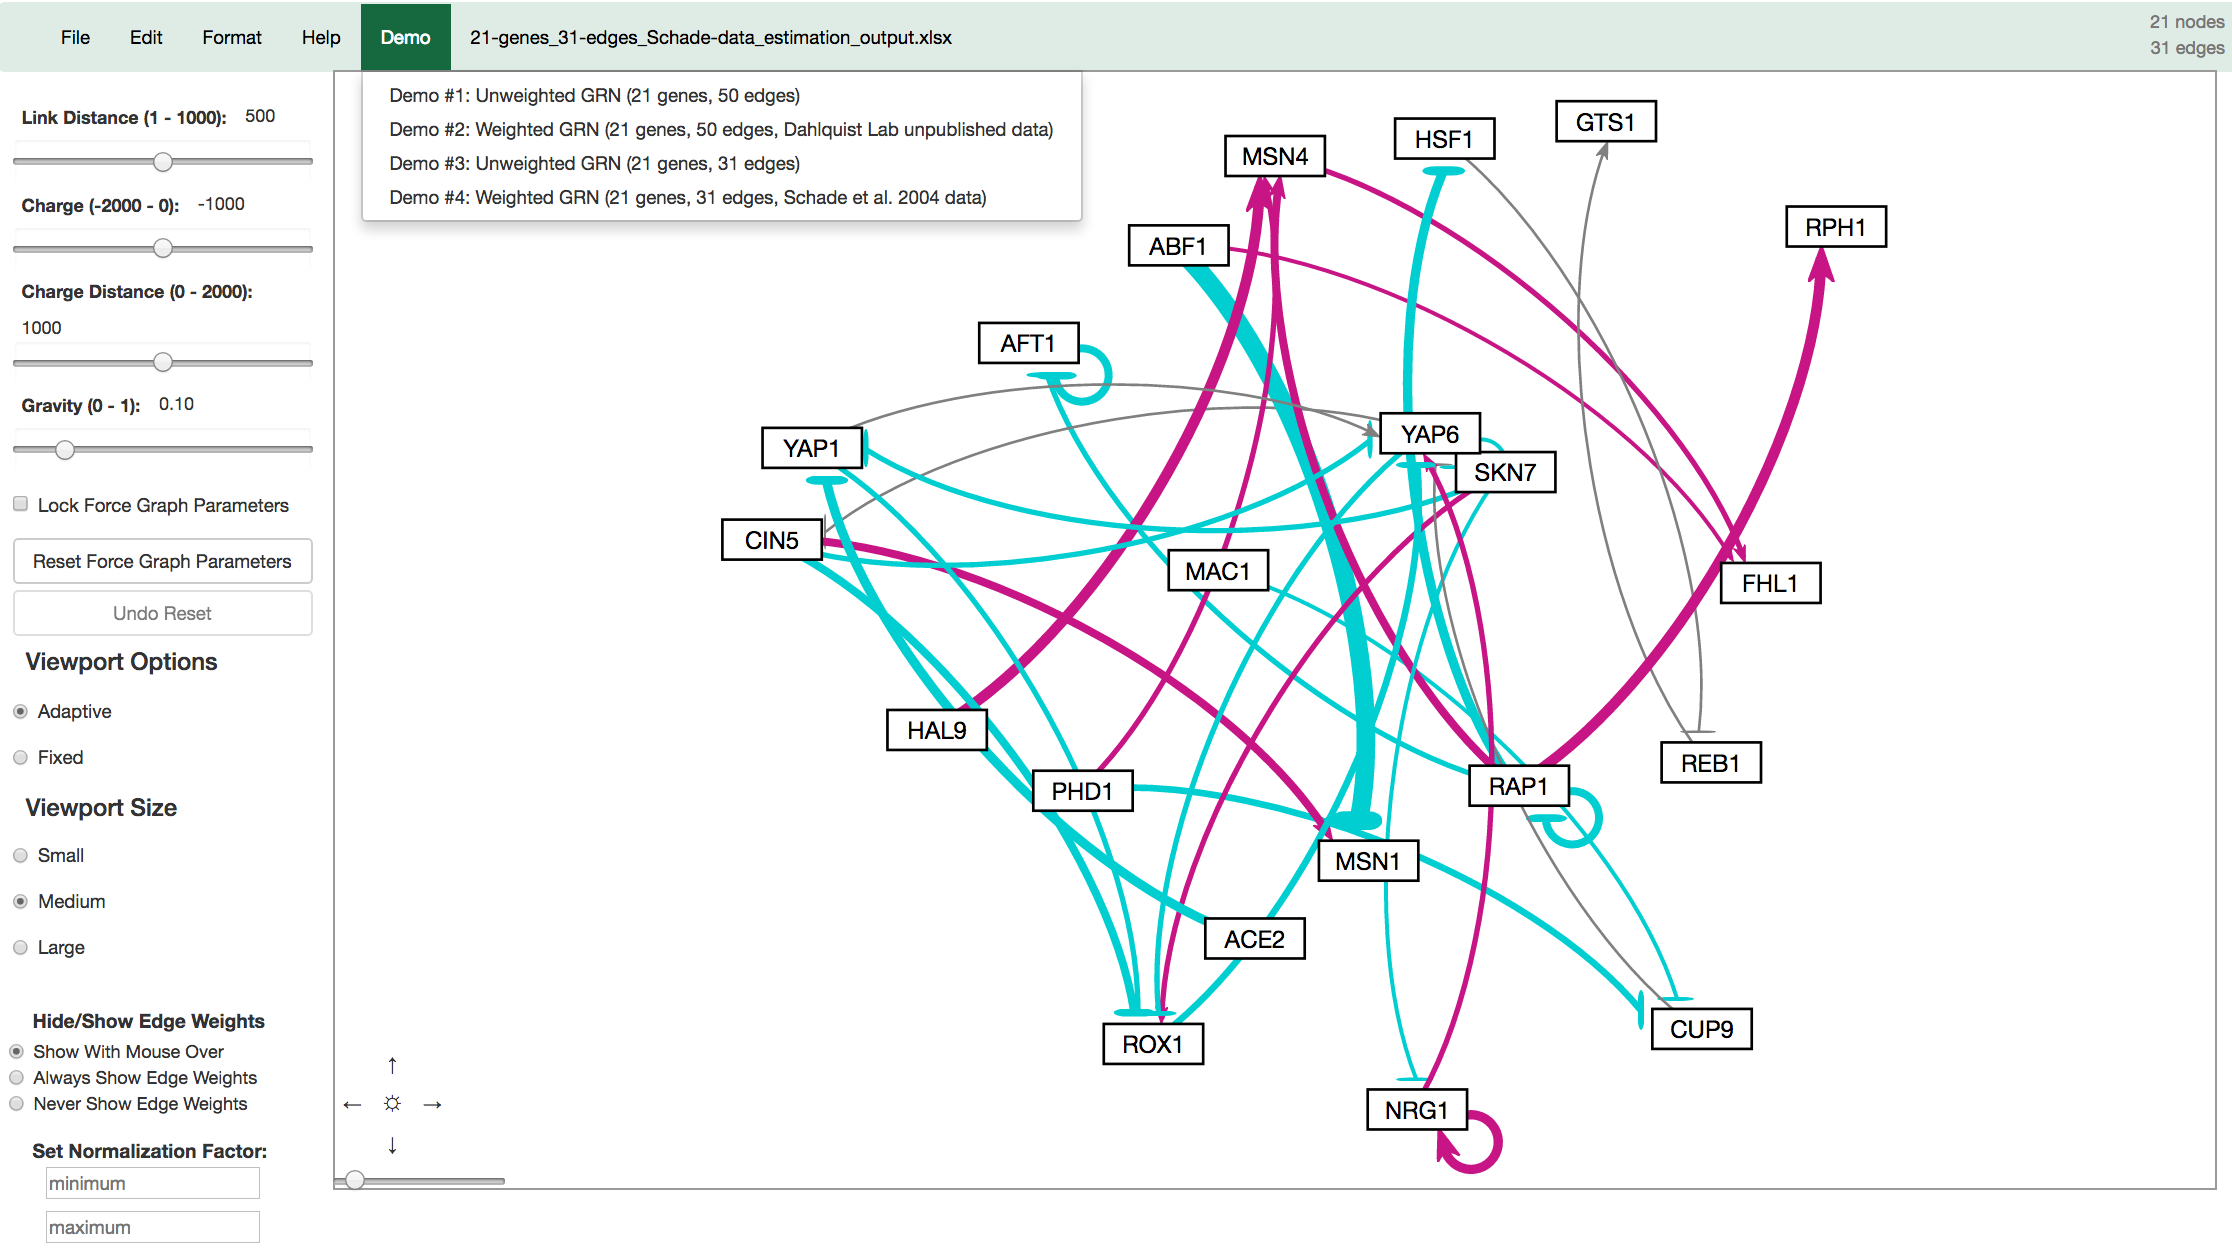
\includegraphics[height=1.5in]{screenshot-auto.png}
        \label{fig:full-screenshot}
    }
    \subfigure[Weighted graph after manual manipulation.]
    {
        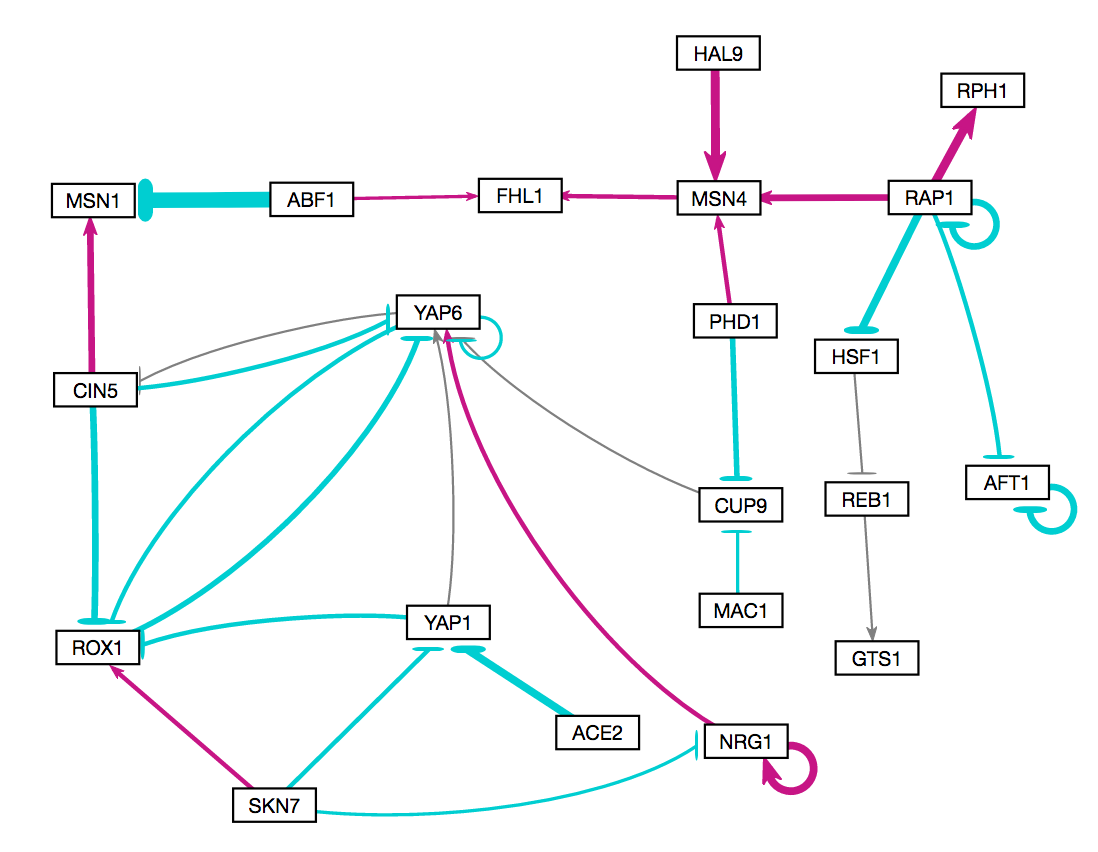
\includegraphics[height=1.5in]{never-weights.png}
        \label{fig:no-weights}
    }
    \subfigure[Weighted graph with edge weights displayed.]
    {
        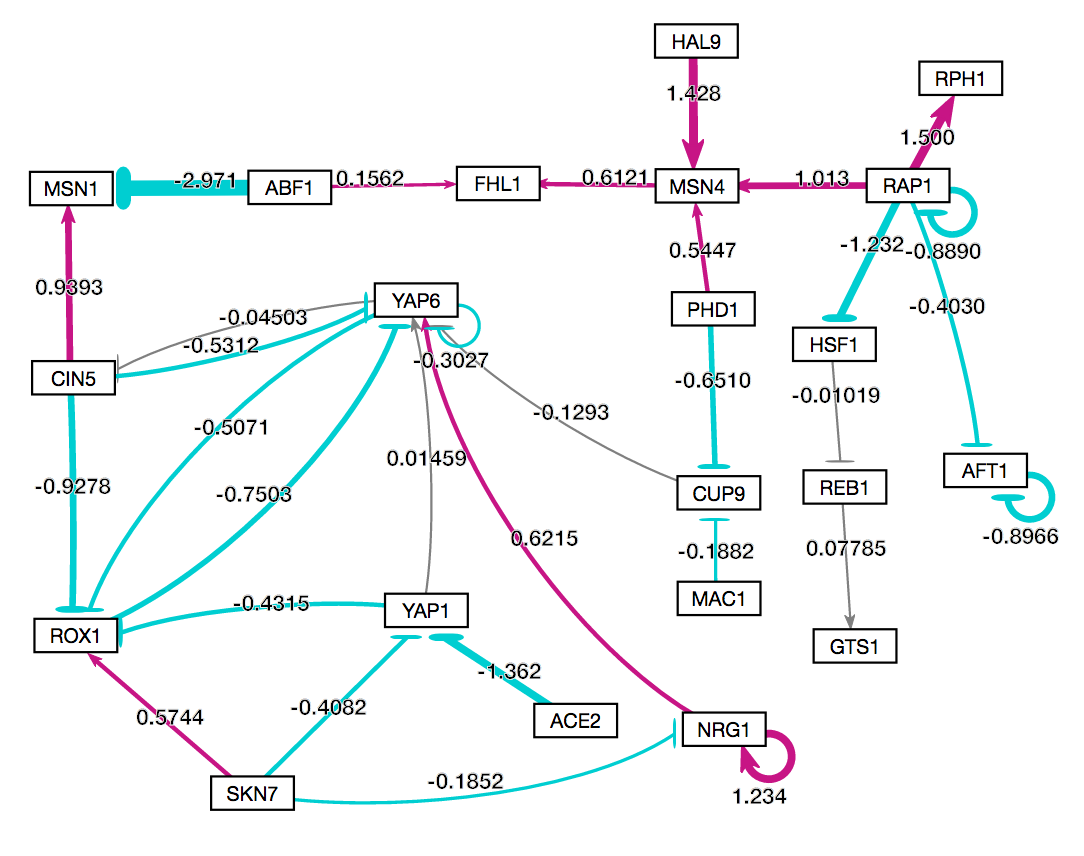
\includegraphics[height=1.5in]{always-weights.png}	
        \label{fig:with-weights}
    }
    \caption{GRNsight v2's automatic graph layout of a 21-gene, 31-edge demo file within an adaptive bounding box (a) allows the gene regulatory network graph to fully relax. Zooming and scrolling options allow the user to see the entire graph when it extends beyond the viewport; (b) the user can manipulate the display of the graph through manual node dragging, and can either hide (b), or show (c) all the weight values, which display on the edges.
    }
    \label{fig:screenshots}
\end{teaserfigure}

\maketitle

\section{Graph Customizations for GRNs}

GRNsight is a web application and service for the interactive visualization of small- to medium-scale gene regulatory networks (GRNs), optimized for use by novice and experienced biologists alike to quickly and easily view unweighted and weighted network graphs \cite{peerj}. Graph visualization in GRNsight is facilitated by the Data-Driven Documents JavaScript library \cite{d3}. D3.js provides data mapping and layout routines which are heavily customized, producint a graph as a Scalable Vector Graphics (SVG) drawing in which D3.js maps gene objects from the JSON representation provided by the web API server onto labeled rectangles. Directed edges are mapped into Bezier curves. The resulting graph is interactive, initially using D3.js's force graph layout algorithm to automatically determine the positions of the gene rectangles, but also allowing the user to manually manipulate the graph by node dragging. Since the release of GRNsight v1, feedback from peer review and the related GRNmap software modeling team \cite{http://kdahlquist.github.io/GRNmap/} have motivated the following improvements in GRNsight v2.

\subsection{Separation of Viewport from Graph Bounding Box}
The default behavior of D3.js's force graph layout algorithm is to give the graph an \emph{a priori} bounding box, which was initially set to fit to a single viewport size. However, the fixed size did not allow for graphs above a relatively small number of nodes to fully come to rest. Nodes would instead bump up against the edge of the bounding box. Thus, we revised the algorithm to provide an option for an adaptive bounding box that could expand beyond the viewport. This allows the graph to expand as far as required for it to converge to a steady state, allowing the force graph parameters to be fully applied. Because of this change, the ability for the user to zoom and scroll the graph within the viewport was also added. The option to utilize the default behavior of a bounding box fixed to the viewport was also retained.

There are three size options for the viewport: small, medium and large. Initially upon loading GRNsight, the best of these preset viewport sizes is chosen using the current size of the browser window. The viewport (and bounding box, if fixed to viewport) can also be custom-fit to the maximize the available space in the browser, beyond these three presets. These settings can be changed at any time. 

\subsection{Edge Weight Value Display Options}
In GRNsight v1, edge weight values were only displayed upon mouse-over of the edge, one value at a time, making it difficult to compare weight values between two edges. In GRNsight v2, the option now exists for users to always show or always hide weights, as well as the default option of viewing weight values only upon mouse-over (Figure~\ref{fig:screenshots}). Edge Options are selected in the sidebar menu, and under the Format dropdown in the menu bar.

\subsection{Graph Normalization}

To allow for the comparison of weighted network graphs, GRNsight v2 adds the option to customize the normalization factor applied to edge thicknesses. By default, GRNsight detects the maximum and minimum edge weight values of a network, and normalizes the data to fit within 12 distinct preset edge thicknesses corresponding to the strength of its regulatory relationship. This ensures that the edges of a weighted graph are visually distinguishable regardless of the absolute values of the weights. However, with this model, a graph with weights in the range \(-1\) to \(1\) could appear the same as a graph with weights in the range \(-10\) to \(10\). By adding the option for user-specified minimum and maximum values, the edge thicknesses can be normalized to consistent values, so the user can compare different graphs on the same scale (Figure~\ref{fig:network-screenshots}).
%
%\begin{figure}[h]
%    \centering
%    \subfigure[Network A]
%    {
%        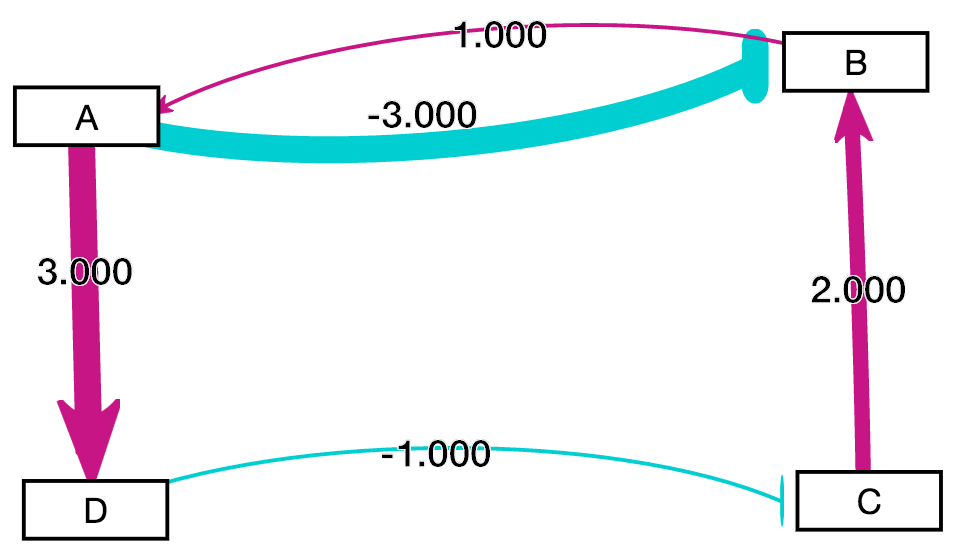
\includegraphics[height=1in]{networkA.png}
 %       \label{fig:networkA}
%    }
%    \subfigure[Network B without Normalization]
%    {
%        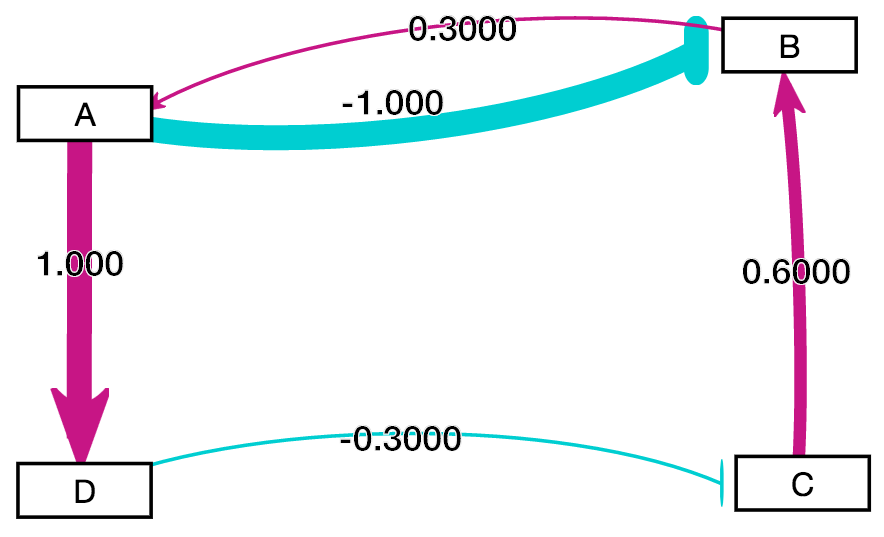
\includegraphics[height=1in]{networkB.png}
%        \label{fig:networkB}
%    }
%    \subfigure[Network B with Normalization]
%    {
%        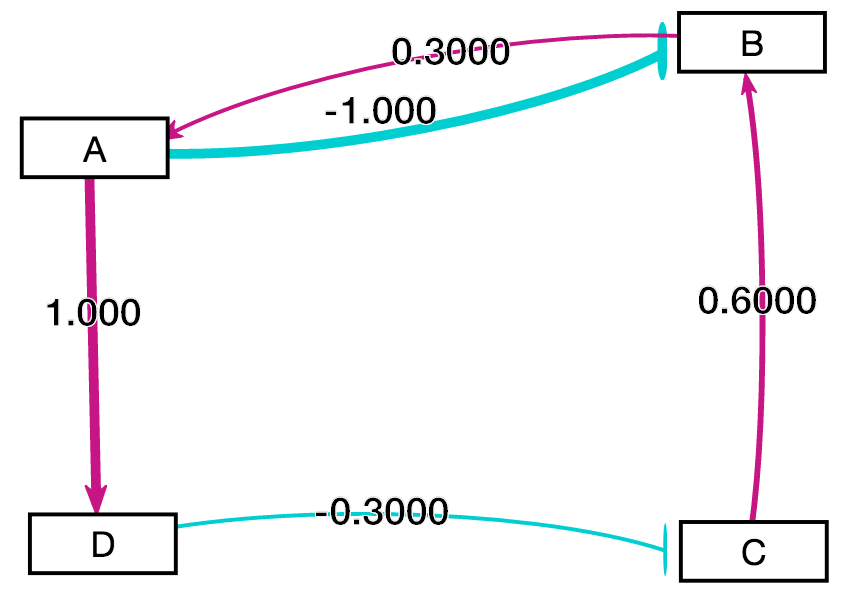
\includegraphics[height=1in]{networkB-normalized.png}	
%        \label{fig:networkB-normalized}
%    }
%    \caption{GRNsight automatically detects the minimum and maximum weights in (a) and (b) to normalize and set edge thicknesses. By overriding the maximum and minimum values of Network B and setting them to \(-3, 3\) in (c), Network B is now normalized to match the scale of Network A. Now the network visualization in (a) and (c) can be directly compared.}
%    \label{fig:network-screenshots}
%\end{figure}

\section{Conclusion and Future Work}
We have successfully built upon GRNsight v1, a web application and service for visualizing small- to medium-scale GRNs that is simple and intuitive to use. GRNsight reads a weighted or unweighted representation of a GRN, and automatically lays out and displays unweighted and weighted network graphs, enabling interpretation of the weight parameters more easily than one could from an adjacency matrix alone. Extensions to GRNsight in v2 have expanded GRNsight's visualization and layout capabilities, giving the user more control over the visual display of the network graph.

GRNsight is in active development, closely interacting with the GRNmap modeling group. We plan to add features to compute and display graph statistics, such as betweenness centrality, and provide different graph layout options, such as a hierarchical or block layout, as well as explore the effectiveness of alternate visualization paradigms for biologist users who are seeking visual insight into GRNs.

\bibliographystyle{ACM-Reference-Format}
\bibliography{siggraph-abstract-review} 

\end{document}
